\section{The DOM: The Basic Unit of IceCube}

\label{subsec:pmt}
\subsection{The Photomultiplier Tube}
The basic unit of the IceCube detector is the \emph{digital optical module}, often referred to simply as the \emph{DOM} \cite{Description-IceCube}.
The DOM is designed around a downward-facing 10 inch R7081-02 photomultiplier tube (\emph{PMT}) from Hammamatsu Photonics \cite{IceCube-PMT,IceCube-PMT-Hammamatsu} and includes onboard electronics for standard operation as shown in Figure~\ref{fig:icecube_dom}. 
Circuit boards are included for data acquisition, control, calibration, comminuications and power conversion as well as for high voltage input from the surface.
The electronics of the DOM are encased in a spherical glass housing designed to withstand the high pressures associated with operation in the glacier of Antarctica.
The PMT is optically coupled to the glass housing in order to minimize distortion of incoming light. 

\begin{figure}
\centering
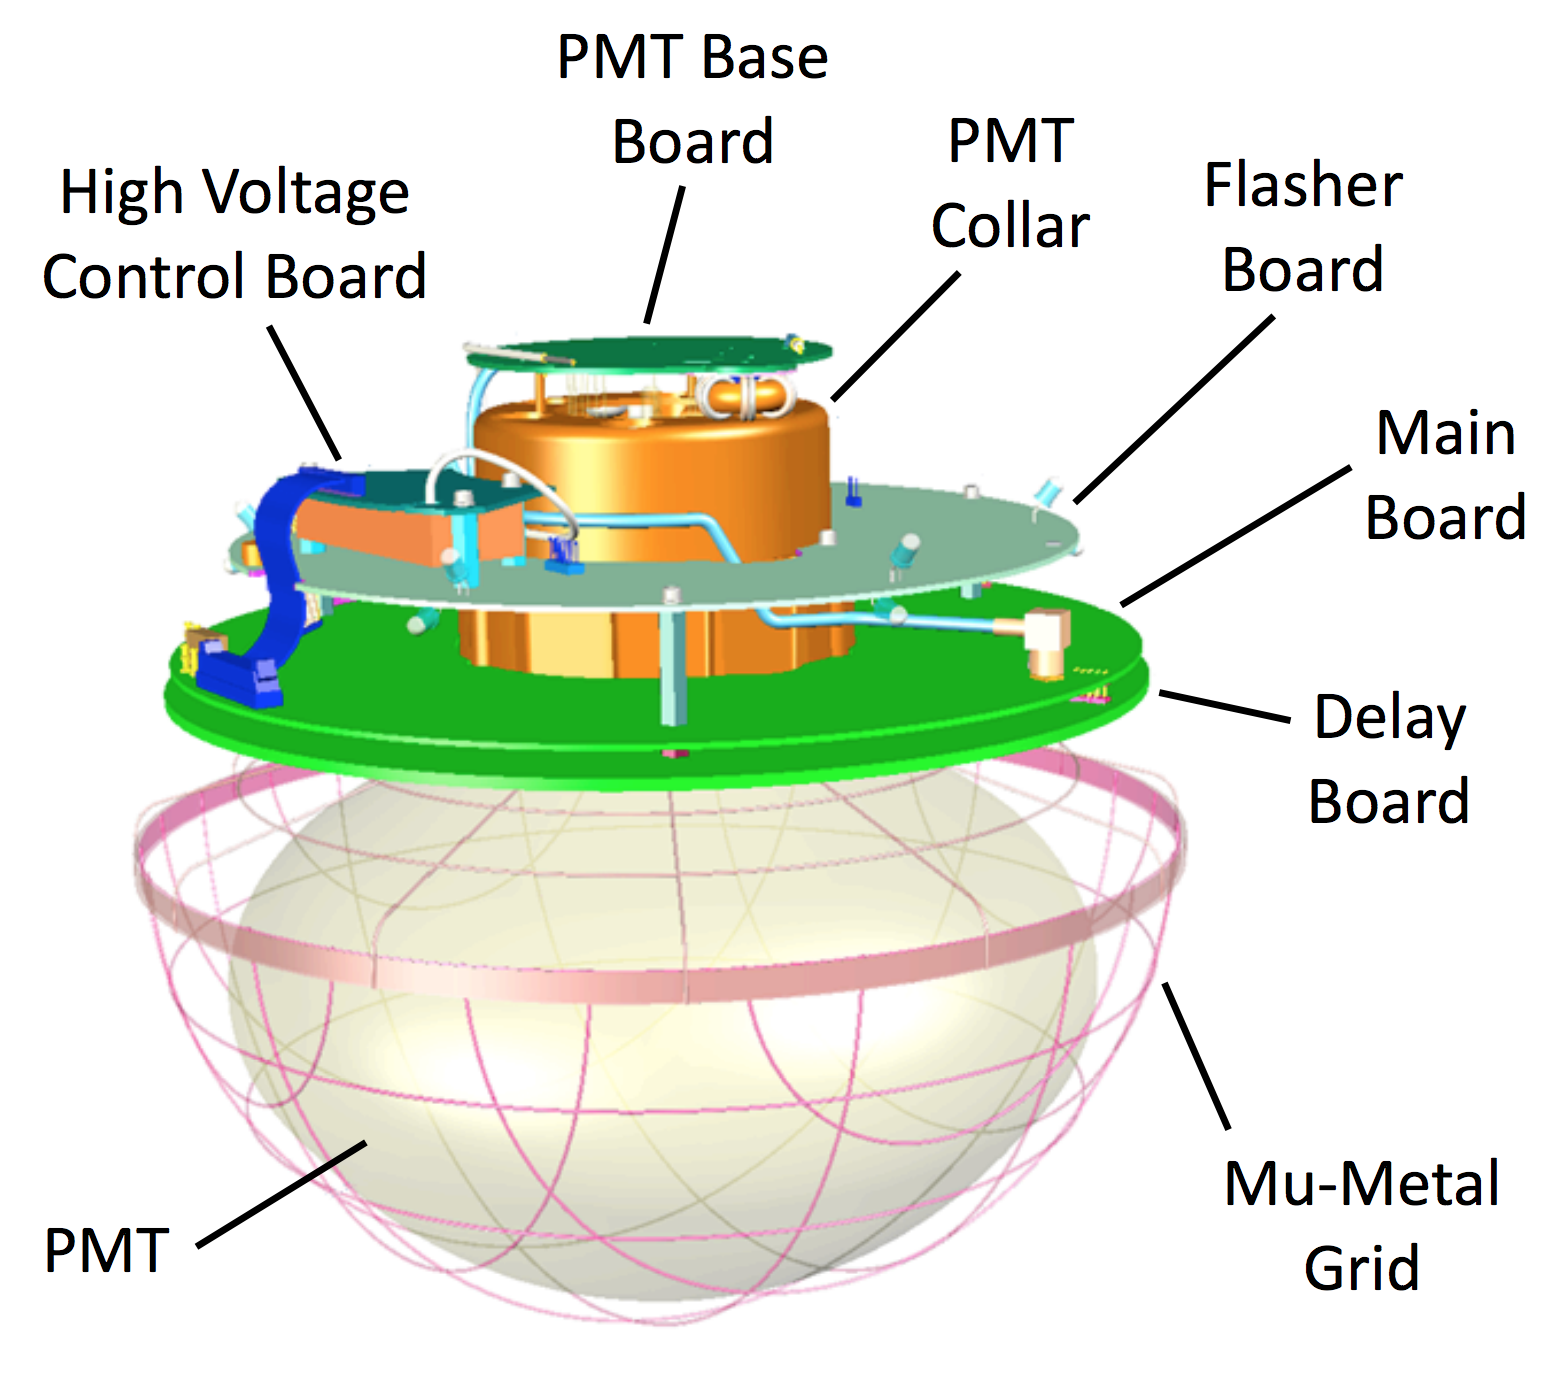
\includegraphics[width=0.4\textwidth]{icecube_dom.png}
\caption{The IceCube DOM contains multiple components, including the PMT itself as well as various electronics necessary for semi-autonomous operation.}
\label{fig:icecube_dom}
\end{figure}

A discriminator onboard the DOM is used to identify signals from the PMT with a voltage threshold corresponding to 0.25 photoelectrons.
Each discriminator crossing begins a \emph{DOM launch}, the lowest level signal available in the IceCube detector containing a digitization of a raw PMT output in the form of a \emph{waveform}.
Information from the PMT is digitized using the fast analog-to-digital converter (\emph{fADC}), which provides binned information at 40 megasamples/second for for the 6.4 microseconds following the initial DOM launch.
Simultaneously, the analog signal is recorded by the onboard custom integrated circuits known as \emph{Analog Transient Waveform Digitizers} (\emph{ATWDs}) for possible high quality digitization.
Launches are recorded in DOM memory while awaiting a decision from the triggering system.

\label{subsec:LC}
\subsection{Local Coincidence}
If any of the notified DOMs also record a launch within a configurable 1 microsecond window, both launches are said to form a \emph{hard local coincidence} (\emph{HLC}) pair.
Nearby DOMs, here defined to be either of the two DOMs above or below the current DOM, are notified of the launch via a signal sent using the \emph{local coincidence} wiring.
In this situation, all DOMs participating in the HLC begin producing higher quality digitizations from the recorded analog signals using the ATWDs.
Launches which fail to satisfy the local coincidence conditions are referred to as \emph{soft local coincidence} (\emph{SLC}) hits.
Launches digitized as part of an HLC pair receive a flag. 
This flag may be used to later identify only those launches which satisfy the local coincident conditions, providing a simple, default method of identifying hits likely to be caused by particle interactions in the detector.

\label{subsec:digitization}
\subsection{Digitization}

\begin{figure}
\centering
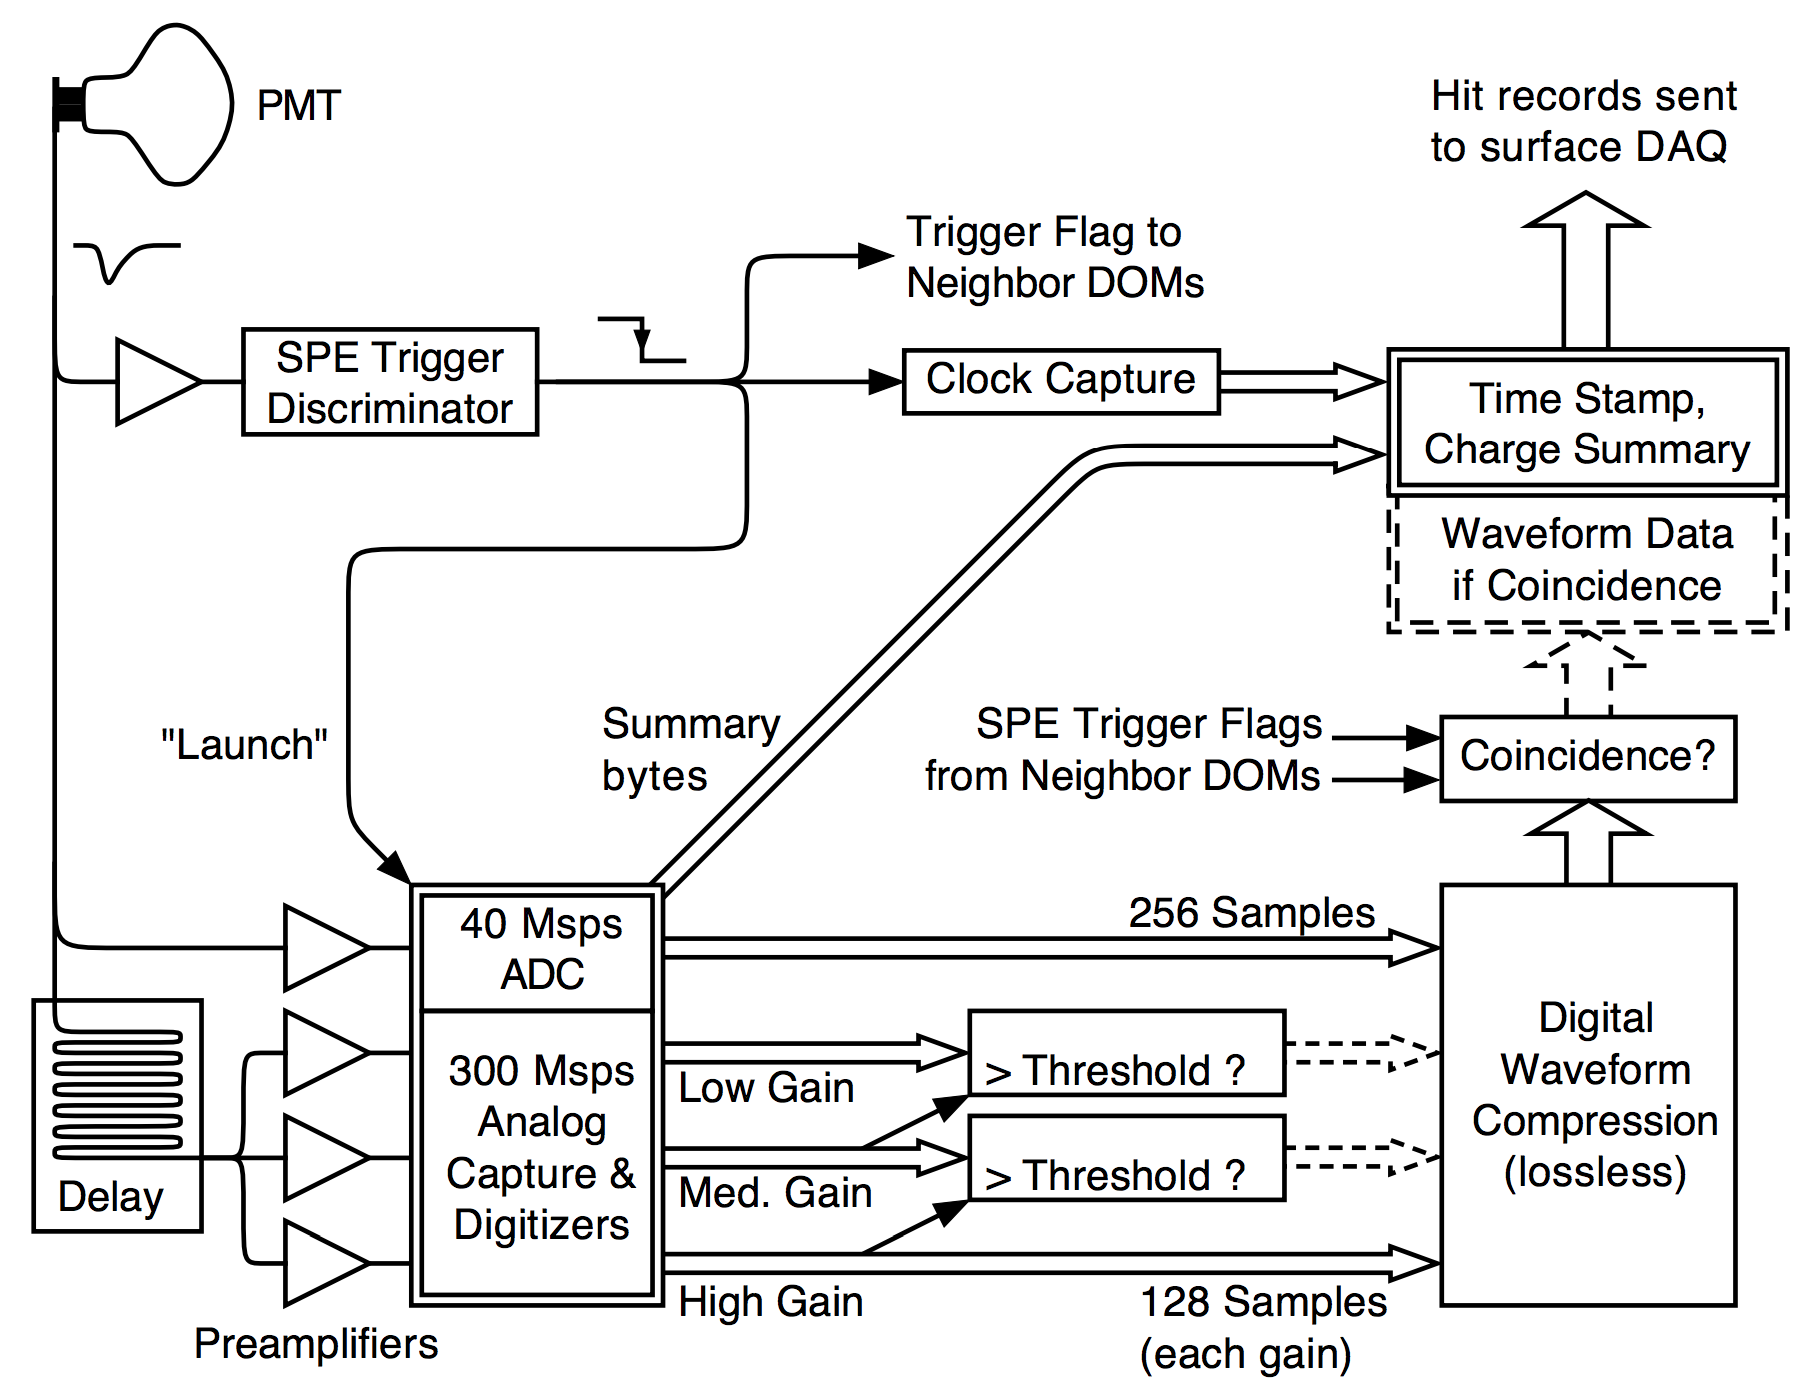
\includegraphics[width=0.6\textwidth]{onboard_trigger.png}
\caption{A schematic diagram of the onboard launch system for the IceCube DOMs. Taken from \cite{Description-IceCube}}
\label{fig:onboard_trigger}
\end{figure}

Signals from the PMT are digitized using a variety of digitizers, shown in Figure~\ref{fig:onboard_trigger}.
Each DOM contains two ATWD chips, each of which has access to three amplifier gain levels in order to cover the dynamic range of the PMT.
The highest gain channel is used for most pulses, although lower gains are used in cases of particularly large pulses in order to avoid loss of information due to saturation of the channel.
The ATWD chips sample the waveform at a rate of 300 megasamples/second with 128 samples per launch, recording a total of 427 nanoseconds.
A 10 meter long delay line embedded in the circuitry of the DOM allows the ATWD to record signals from approximately 75 nanoseconds before the discriminator crossing.

When digitizing a signal, the ATWD chip experiences 29 microseconds of deadtime \cite{Description-IceCube}. 
During this time, the secondary ATWD is available to record further pulses, resulting in a total average fractional deadtime per DOM of $\mathtt{2.2 \times 10^{-5}}$ seconds/second.

\begin{figure}
\centering
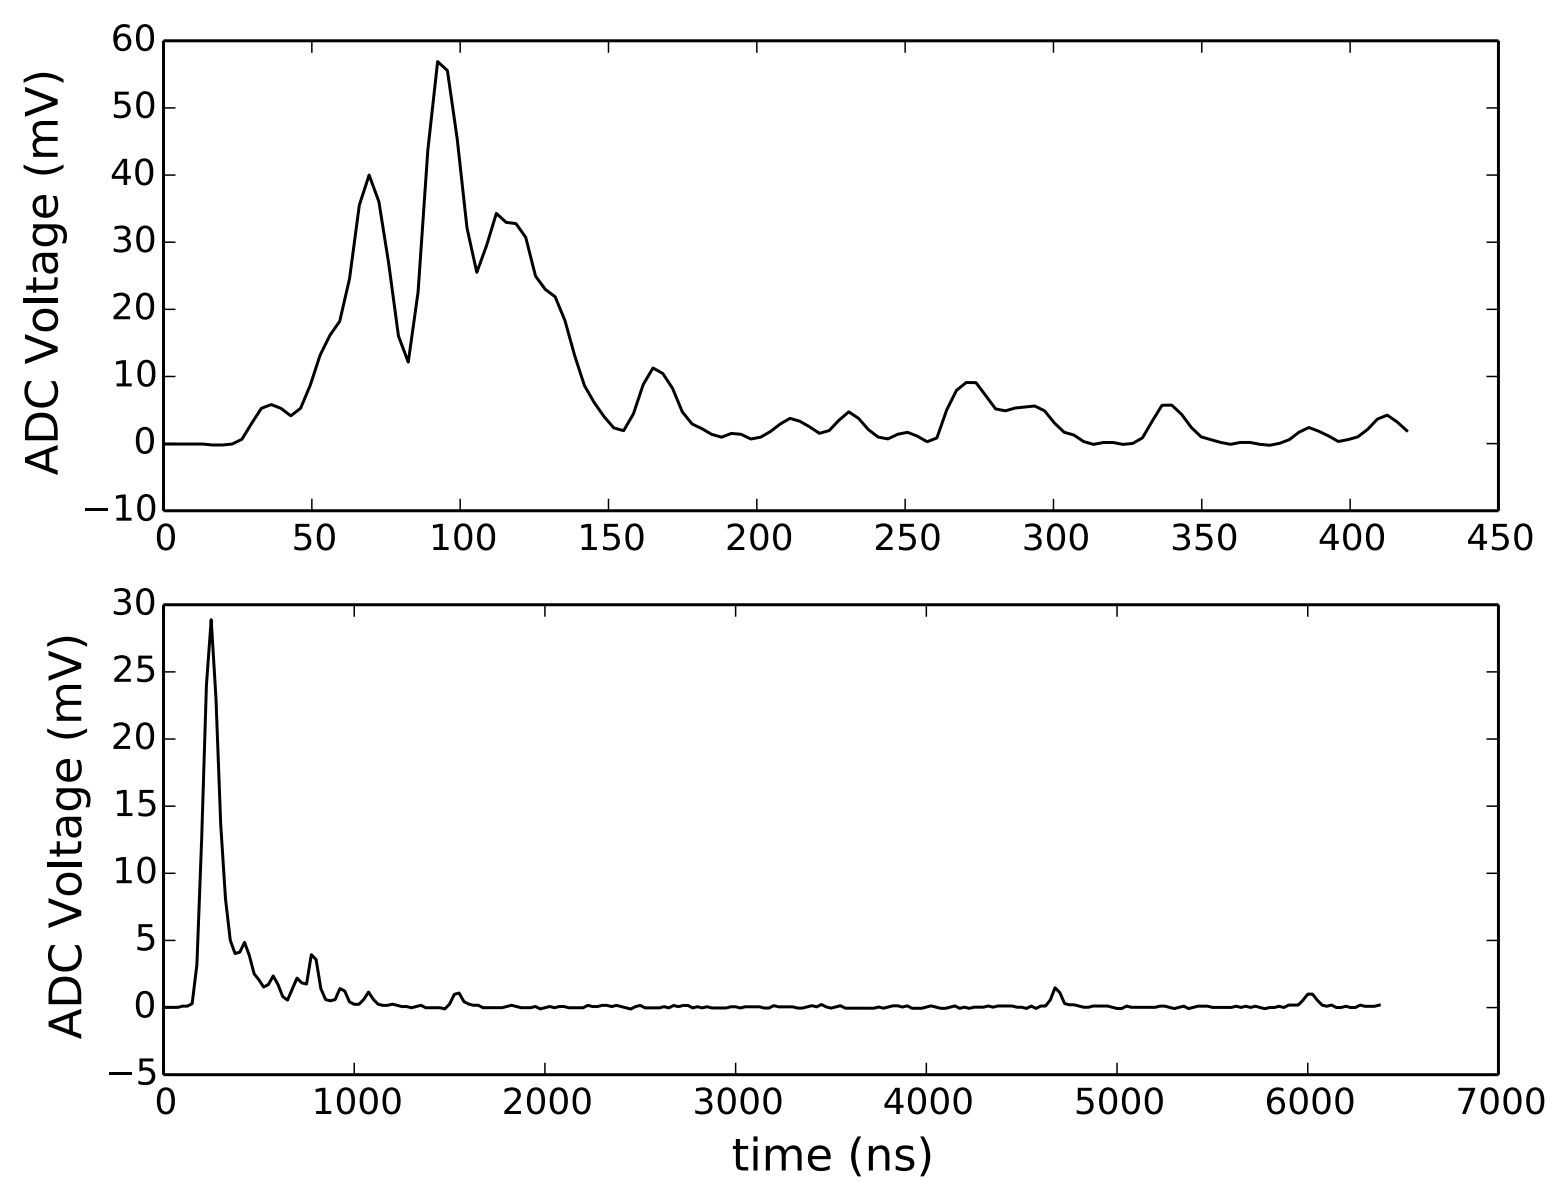
\includegraphics[width=0.6\textwidth]{icecube_waveforms.png}
\caption{Examples of the ATWD (top) and FADC (bottom) waveforms output from an IceCube PMT. Taken from \cite{Description-IceCube}}
\label{fig:waveforms}
\end{figure}

Examples of digitized waveforms from the ATWD and fADC are shown in Figure~\ref{fig:waveforms}.

\subsection{Triggering in IceCube}
Digitized versions of the waveforms are transmitted from the DOM to the IceCube physics data acquisition system (\emph{pDAQ}) for use in trigger and event building.
The most common type of trigger used in IceCube analyses is the \emph{Simple Majority Trigger} or \emph{SMT}. 
This trigger is designed to look for coincidences between DOMs using HLC launches.
Each of the SMTs is defined by three fundamental configurations: a DOMSet, which lists the DOMs available for use in the trigger conditions; a threshold number of HLC launches before the trigger fires; and a time window length in which the HLC are required to coexist.

Once all triggers are identified, a \emph{global trigger} is defined. 
This consists of the superset of all triggers occurring within 10 microseconds of one another.
All detector readout enclosed within the global trigger as well as additional information within an additional 10 microseconds both before and after the trigger is combined into a single \emph{event}.

